% 使用 XeLaTeX + BibTeX 编译
% xelatex main.tex && bibtex main.aux && xelatex main.tex && xelatex main.tex

% 可使用 overleaf 在线编译,也可使用在本地使用 texlive 进行编译

% 清除临时文件
% rm main.bbl main.blg main.toc main.out main.aux main.log chap/*.aux

% 有问题可通过邮件或 iMessage 联系: zqye@quicy.cn

\RequirePackage{amsthm}
\documentclass[fontset=fandol, ugly]{pkuthss}
  % 学位论文模式  ugly    (默认打开,请保留)
  % 盲审模式      blind   (默认关闭)
  % 字体库        fontset
  %   auto | windows | windows@overleaf | mac | fandol | ubuntu | none
  % windows*, mac为商业字体,如需使用请遵循相应版权协议(默认下overleaf中不可用)
  % fandol与windows效果相近,但字符库偏少,推荐使用(默认);
  % ubuntu字体效果偏差较大; 设为none时需自行配置字体集;
\usepackage{natbib}
\let\openbox\relax
\usepackage{enumitem,fancyvrb}
\usepackage{booktabs,multirow,longtable,makecell}
\RecustomVerbatimEnvironment{Verbatim}{Verbatim}{frame = single, tabsize = 4, fontsize=\footnotesize}
\renewcommand{\v}[1]{\boldsymbol{#1}}
\newcommand\pkg[1]{\textsf{#1}}
\raggedbottom
\setlength{\hfuzz}{3pt}
\ctexset{
	linestretch = 2\ccwd,
	contentsname = {Contents},
	listfigurename = {List of Figures},
	listtablename = {List of Tables},
	figurename = {Figure},
	tablename = {Table},
	indexname = {Index},
	appendixname = {Appendix},
	part/name = {\partname\space},
	part/number = {\thepart},
	chapter/name = {\chaptername\space},
	chapter/number = {\thechapter}
}

\newcommand{\myemph}[1]{\emph{\textcolor{red}{#1}}}
\newcommand{\unemph}[1]{\textup{\textcolor{black}{#1}}}
\newcommand{\docversion}{v1.7.4}
\usepackage{pdfpages}
\usepackage{amsmath}
\allowdisplaybreaks[4]
\usepackage{mathrsfs}
\usepackage{amsfonts}
\usepackage{dsfont}
\usepackage{bm}
\usepackage{bbm}
\usepackage{comment}
\usepackage{graphicx}
\usepackage{multirow}
\usepackage{indentfirst}
\usepackage{arydshln}
\usepackage{shorttoc}
\usepackage[plain,ruled,algochapter]{algorithm2e}
\usepackage{threeparttable}
\graphicspath{{img/}}
\newcommand{\red}{\color{red}}
\newcommand{\blue}{\color{blue}}
\newcommand{\green}{\color{green}}
\newtheorem{definition}{Definition}[chapter]
\newtheorem{theorem}{Theorem}[chapter]
\newtheorem{lemma}{Lemma}[chapter]
\newtheorem{proposition}{Proposition}[chapter]
\newtheorem{assumption}{Assumption}[chapter]
\newtheorem{remark}{Remark}[chapter]
\newtheorem{corollary}{Corollary}[chapter]
\theoremstyle{remark}
\newtheorem{example}{Example}[chapter]


\newlength{\bibitemsep}\setlength{\bibitemsep}{.2\baselineskip plus .05\baselineskip minus .05\baselineskip}
\newlength{\bibparskip}\setlength{\bibparskip}{0pt}
\let\oldthebibliography\thebibliography
\renewcommand\thebibliography[1]{%
	\oldthebibliography{#1}%
	\setlength{\parskip}{\bibitemsep}%
	\setlength{\itemsep}{\bibparskip}%
}

\def\bibfont{\zihao{5}\linespread{1.27}\selectfont}

\pkuthssinfo{
	cthesisname = {博士学位论文},
 	thesiscover = {博士研究生学位论文},
	ethesisname = {Doctoral Dissertation},
	ctitle = {博士学位论文英文模板 (XeLaTeX + BibTeX)},
	etitle = {Template for Doctoral Dissertation (XeLaTeX + BibTeX)},
	cauthor = {姓名},
	eauthor = {Author Name},
	studentid = {********},
	date = {\zhdigits{2022}\ \ 年\ \ \zhnumber{5}\ \ 月},
	school = {数学科学学院},
	cmajor = {统计学}, 
	emajor = {Statistics},
	direction = {研究方向},
	cmentor = {XXXX\ \ 教授}, 
	ementor = {Prof.\ XXXX},
	ckeywords = {XXX,XXX,XXX。}, 
	ekeywords = {XXX, XXX, XXX.}
}
\hypersetup{colorlinks = true, allcolors = blue}

\begin{document}
	\frontmatter
	\pagestyle{empty}
	\maketitle
	\cleardoublepage
	\chapter*{版权声明}
\thispagestyle{empty}

% 替换门户下载pdf
\begin{textblock}{1}(-0.8,-0.08)
    \colorbox{white}{
        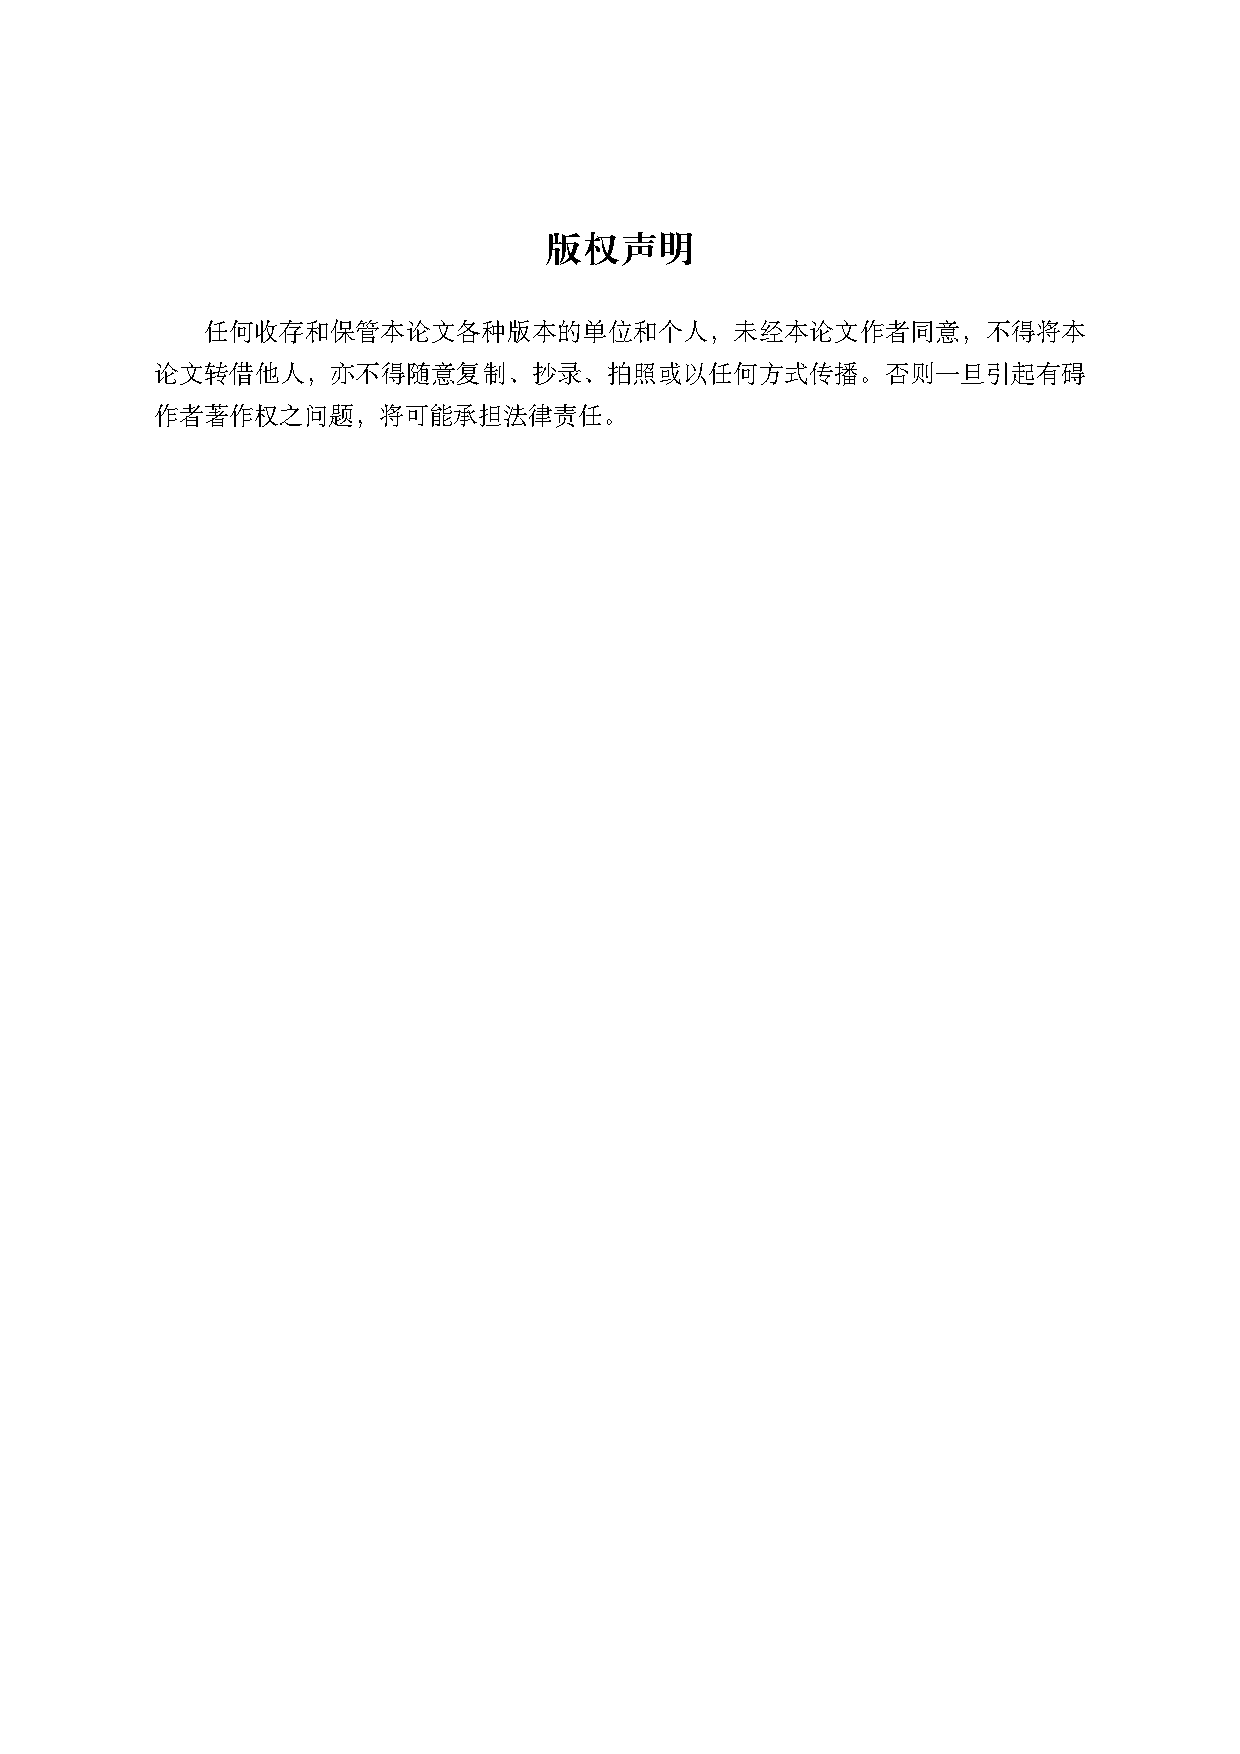
\includegraphics[height = 1.2448\textheight]{bqsm.pdf}
    }
\end{textblock}

	\cleardoublepage
	\pagestyle{plain}
	\setcounter{page}{0}
	\pagenumbering{Roman}
	% 中文摘要
\begin{cabstract}
    在\href{https://www.overleaf.com/latex/templates/2021-peking-university-master-thesis-template-iofu728-pkuthss/rwfvbkpzydpf}{北京大学硕士学位论文模板 (iofu728)} 的基础上进行了以下改进:
    \begin{itemize}
        \item 将中文模板更改为英文模板。
        \item 将参考文献编译器从 Biber 更改为 BibTeX,避免原先的 textcite 等。
        \item 增加学位论文答辩委员会名单、博士学位论文答辩委员会决议书、提交终版学位论文承诺书 (在模板中均由版权声明代替,需要替换你自己的文件)。
        \item 使 enumitem 支持 (1)、(a)、(i) 等格式,避免原先的 arabic, roman 等。
        \item 增加定理类环境和证明环境,增加插入表格、算法、图片等代码。
    \end{itemize}

    \bigskip

    有任何疑问、建议、反馈可以通过邮件或 iMessage 联系我: zqye@quicy.cn。
    
    \bigskip
    
    打个广告,高效使用 LaTeX 可参考:

    \url{https://quicy.notion.site/LaTeX-6be09d441a594bed84d59dba2b254034}


\end{cabstract}

% 英文摘要
\begin{eabstract}
English abstract.
\end{eabstract}
	\tableofcontents
	\mainmatter
	\chapter{Introduction}\label{chapter: introduction}

	\chapter{Title}\label{chapter: 2}
\section{Theorem Environment}
\begin{theorem}\label{theorem: convergence}
    Let $X_1,X_2,\dots$ be pairwise independent identically distributed random variables with $EX_i<\infty$. Let $EX_i=\mu$ and $S_n=X_1+\cdots+X_n$. Then $S_n/n\rightarrow\mu$ a.s. as $n\rightarrow\infty$.
\end{theorem}

\begin{lemma}\label{lemma: convergence}
    Let $X_1,X_2,\dots$ be pairwise independent identically distributed random variables with $EX_i<\infty$. Let $EX_i=\mu$ and $S_n=X_1+\cdots+X_n$. Then $S_n/n\rightarrow\mu$ a.s. as $n\rightarrow\infty$.
\end{lemma}

\begin{definition}\label{definition: convergence}
    Let $X_1,X_2,\dots$ be pairwise independent identically distributed random variables with $EX_i<\infty$. Let $EX_i=\mu$ and $S_n=X_1+\cdots+X_n$. Then $S_n/n\rightarrow\mu$ a.s. as $n\rightarrow\infty$.
\end{definition}

\begin{proposition}\label{proposition: convergence}
    Let $X_1,X_2,\dots$ be pairwise independent identically distributed random variables with $EX_i<\infty$. Let $EX_i=\mu$ and $S_n=X_1+\cdots+X_n$. Then $S_n/n\rightarrow\mu$ a.s. as $n\rightarrow\infty$.
\end{proposition}

\begin{assumption}\label{assumption: convergence}
    Let $X_1,X_2,\dots$ be pairwise independent identically distributed random variables with $EX_i<\infty$. Let $EX_i=\mu$ and $S_n=X_1+\cdots+X_n$. Then $S_n/n\rightarrow\mu$ a.s. as $n\rightarrow\infty$.
\end{assumption}

\begin{remark}\label{remark: convergence}
    Let $X_1,X_2,\dots$ be pairwise independent identically distributed random variables with $EX_i<\infty$. Let $EX_i=\mu$ and $S_n=X_1+\cdots+X_n$. Then $S_n/n\rightarrow\mu$ a.s. as $n\rightarrow\infty$.
\end{remark}

\begin{corollary}\label{corollary: convergence}
    Let $X_1,X_2,\dots$ be pairwise independent identically distributed random variables with $EX_i<\infty$. Let $EX_i=\mu$ and $S_n=X_1+\cdots+X_n$. Then $S_n/n\rightarrow\mu$ a.s. as $n\rightarrow\infty$.
\end{corollary}

\begin{example}\label{example: convergence}
    Let $X_1,X_2,\dots$ be pairwise independent identically distributed random variables with $EX_i<\infty$. Let $EX_i=\mu$ and $S_n=X_1+\cdots+X_n$. Then $S_n/n\rightarrow\mu$ a.s. as $n\rightarrow\infty$.
\end{example}

\begin{proof}[Proof of Theorem \ref{theorem: convergence}]
    Proof of the theorem.
\end{proof}

\section{Enumerate}

\begin{itemize}
    \item a.
    \item b.
\end{itemize}

\begin{enumerate}
    \item 1.
    \item 2.
\end{enumerate}

\begin{enumerate}[(1)]
    \item (1).
    \item (1).
\end{enumerate}

\begin{enumerate}[(a)]
    \item 1
    \item 2
\end{enumerate}

\section{Algorithm}
\begin{algorithm}[htb]
    \SetAlgoLined
    {\bf Initialization:} $S=\varnothing$.
        
    \For{$i=1,\ldots,N$}{
    Generate a Bernoulli variable $R_i\sim\text{Bernoulli}(p_i)$\;
    \If {$R_i=1$}{ Update $S=S\cup\{(\bm {x}_{i},y_{i},p_{i})\}$.}{}
    }
    \caption{Algorithm Caption}
    \label{algorithm: algorithm}
\end{algorithm}

\section{Table}

\begin{table}[htb]
    \caption{Table Caption.}
    \centering
    \begin{threeparttable}
    \setlength{\tabcolsep}{21mm}{ % 控制表格长度
    \begin{tabular}{lll}
        \hline
        Col~1 & Col~2 & Col~3 \\
        \hline
        1.98 & 2.14 & 4.15 \\
        2.18 & 1.90 & 1.45 \\
        \hline
    \end{tabular}}
    \begin{tablenotes}[para,flushleft]
        \footnotesize{footnote}
    \end{tablenotes}
    \end{threeparttable}
    \label{table: label}
\end{table}

\section{Figure}

\begin{figure}[htb]
    \centering
    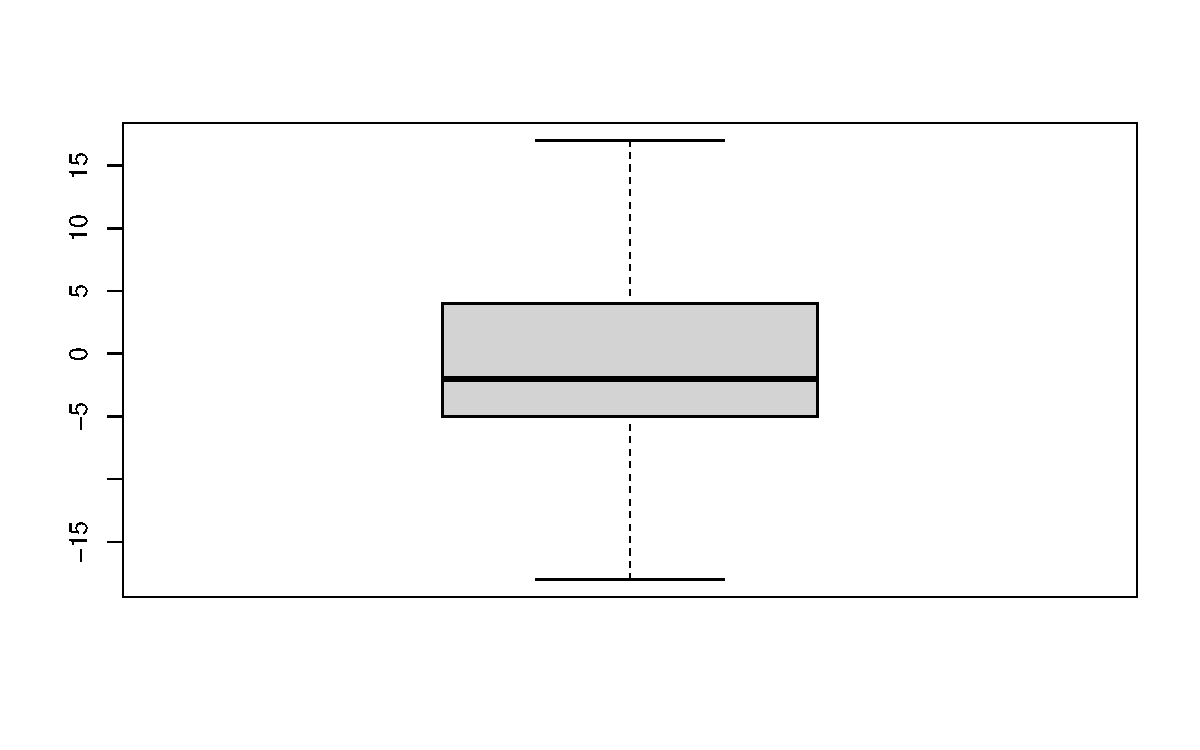
\includegraphics[width=0.95\textwidth]{boxplot}
    \caption{Caption}
    \label{figure: 1}
\end{figure}

\begin{figure}[htp]
    \centering
    \begin{subfigure}{0.49\textwidth}
      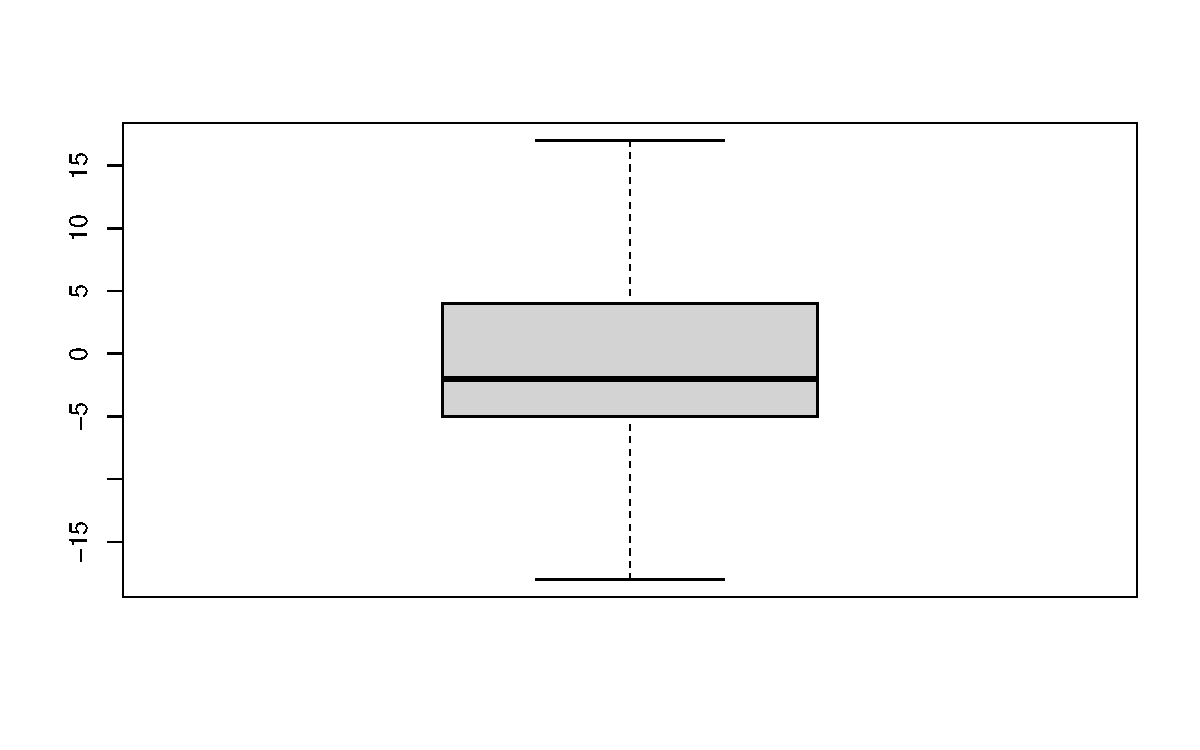
\includegraphics[width=\textwidth]{boxplot}
      \caption{1.}
    \end{subfigure}
    \begin{subfigure}{0.49\textwidth}
      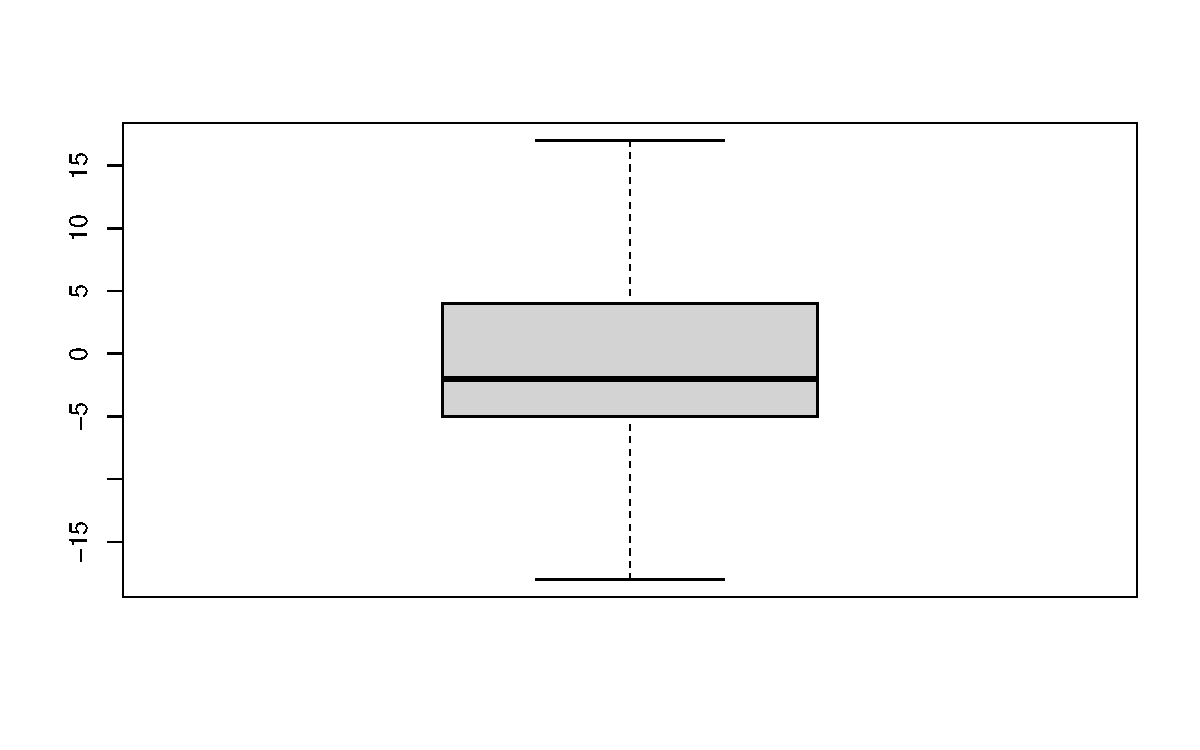
\includegraphics[width=\textwidth]{boxplot}
      \caption{2.}
    \end{subfigure}
    \caption{Caption}
    \label{figure: 2}
\end{figure}
  
\begin{figure}[htb]
    \centering
    \begin{subfigure}{0.49\textwidth}
      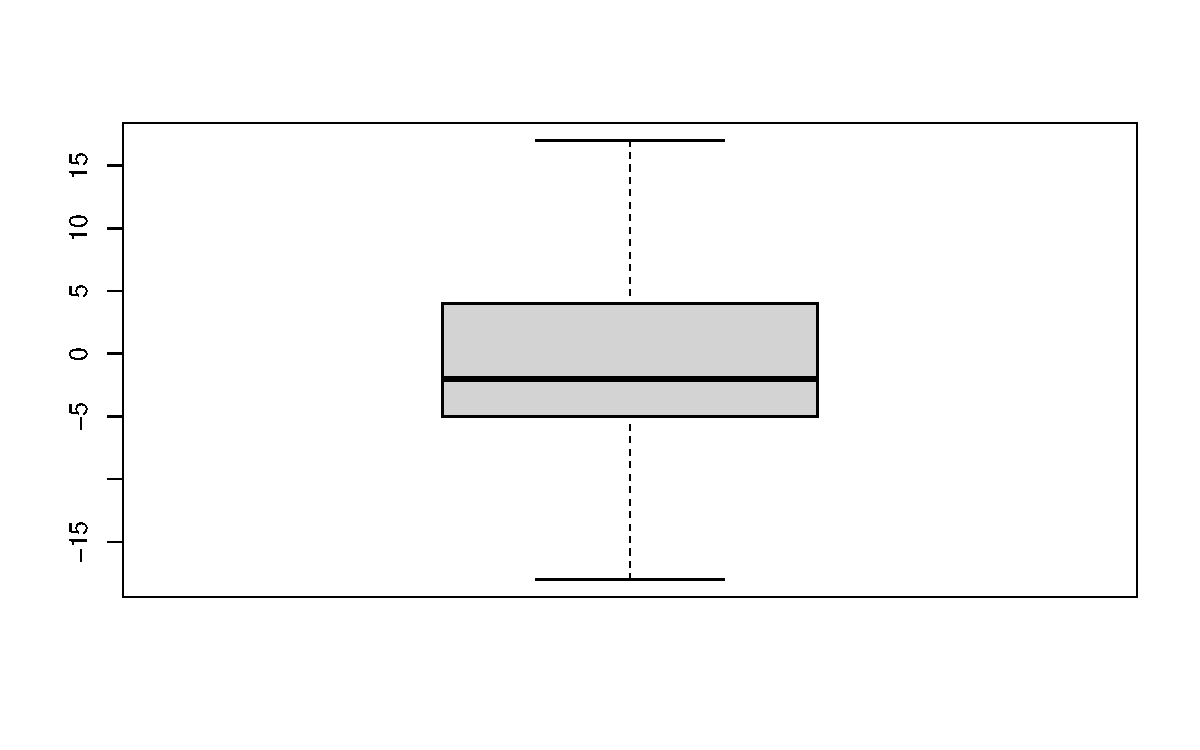
\includegraphics[width=\textwidth]{boxplot}
      \caption{1.}
    \end{subfigure}
    \begin{subfigure}{0.49\textwidth}
      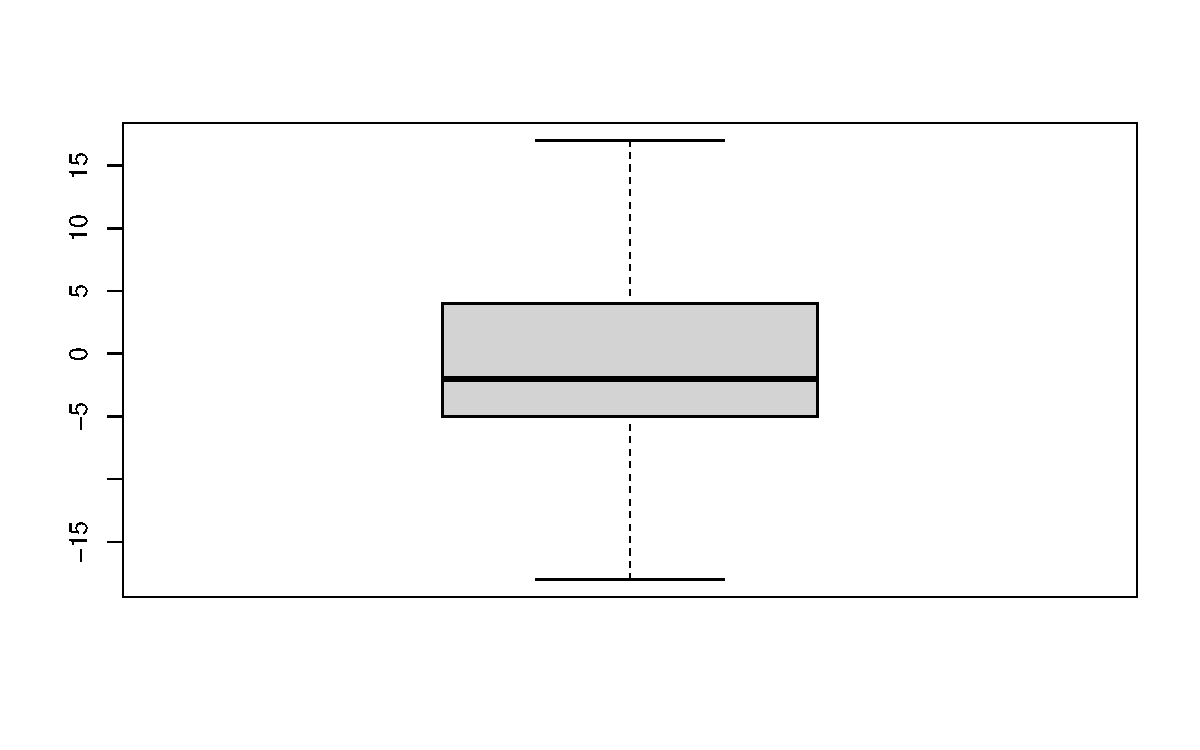
\includegraphics[width=\textwidth]{boxplot}
      \caption{2.}
    \end{subfigure}\\[1mm]
    \begin{subfigure}{0.49\textwidth}
      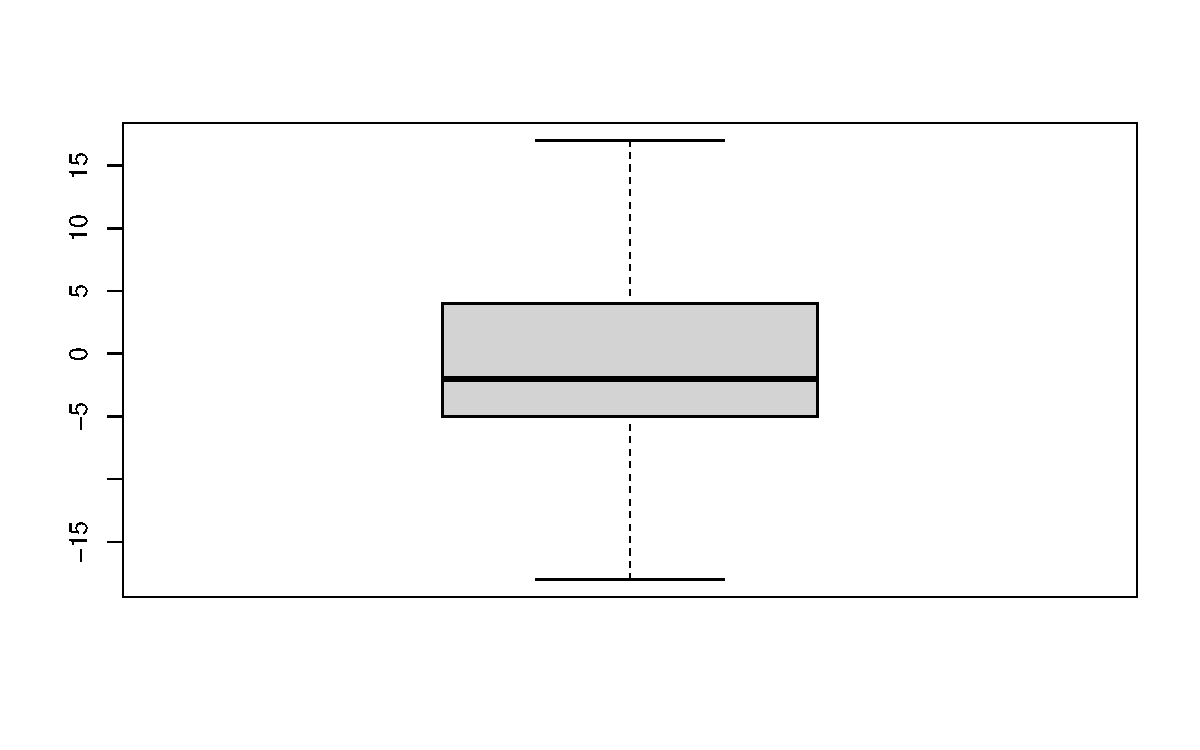
\includegraphics[width=\textwidth]{boxplot}
      \caption{3.}
    \end{subfigure}
    \begin{subfigure}{0.49\textwidth}
      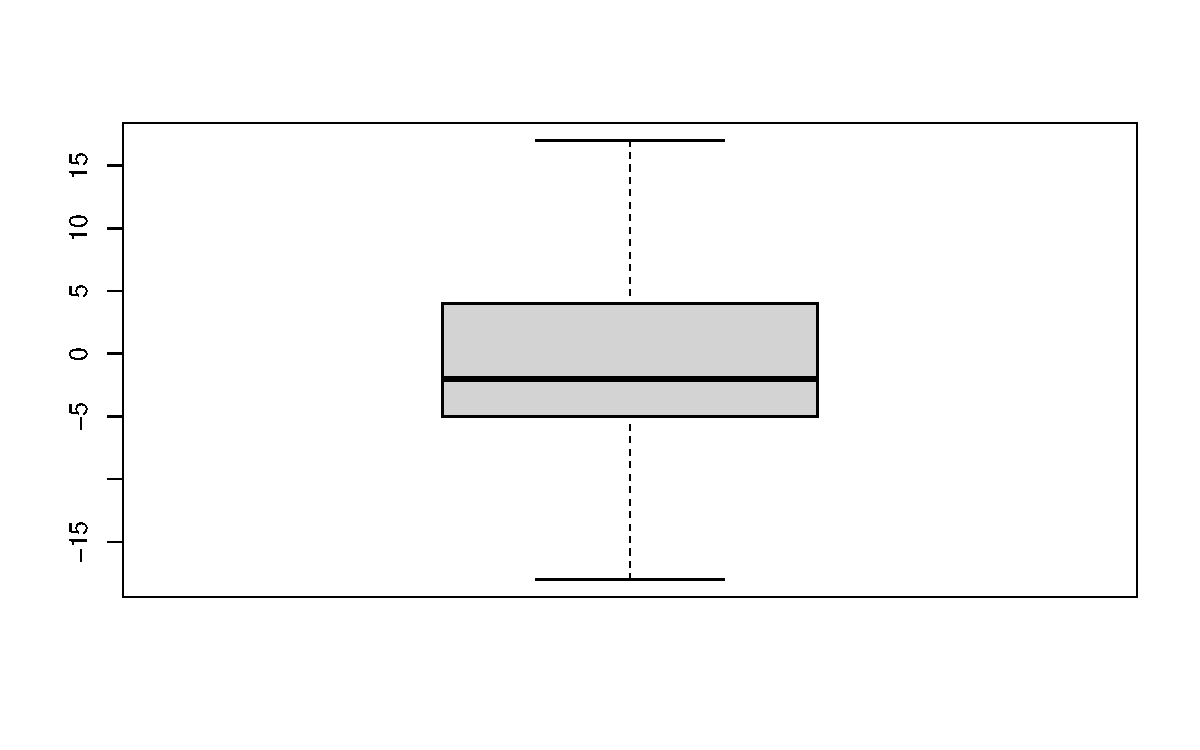
\includegraphics[width=\textwidth]{boxplot}
      \caption{4.}
    \end{subfigure}\\[1mm]
    \caption{Figure.}
    \label{figure: 3}
\end{figure}

\section{Add References}
Author year style: \cite{xue2020online}, \citep{xue2020online}.

	\chapter{Title}\label{chapter: 3}
	\chapter{Title}\label{chapter: 4}
	\chapter{Conclusion}\label{chapter: conclusion}

    \appendix

    \renewcommand{\bibname}{References}
	% author-year 格式的参考文献
	\bibliographystyle{apalike}
	% numeric 格式的参考文献
	% \bibliographystyle{abbrv}
	
	% 你也可以更改为其他 style,参考 https://www.overleaf.com/learn/latex/Bibtex_bibliography_styles
	\bibliography{reference}
	\addcontentsline{toc}{chapter}{References}
    \backmatter
    \chapter{Publications}

\zihao{5}
\noindent \hangafter=1
\setlength{\hangindent}{3em} Xue, Y., Wang, H., Yan, J., and Schifano, E. D. (2020). An online updating approach for testing the proportional hazards assumption with streams of survival data. {\it Biometrics}, 76(1): 171--182.

\noindent \hangafter=1
\setlength{\hangindent}{3em} Xue, Y., Wang, H., Yan, J., and Schifano, E. D. (2020). An online updating approach for testing the proportional hazards assumption with streams of survival data. {\it Manuscript.}

	\zihao{-4}

\chapter{Acknowledgment}

都看到这了,不如打个赏吧 2333333333.
\begin{figure}[htp]
    \centering
    \begin{subfigure}{0.49\textwidth}
      
\includegraphics[width=\textwidth]{alipay}
      \caption{支付宝}
    \end{subfigure}
    \begin{subfigure}{0.49\textwidth}
      
\includegraphics[width=\textwidth]{wechat}
      \caption{微信}
    \end{subfigure}
    \caption*{打赏了哈.}
    \label{figure: pay}
\end{figure}

	\ctexset{section = {
	format+ = {\centering}, beforeskip = {40bp}, afterskip = {15bp}
}}
\specialchap{北京大学学位论文原创性声明和使用授权说明}
\pagestyle{empty}
% 替换门户下载pdf
\begin{textblock}{1}(-0.8,-0.08)
    \colorbox{white}{
        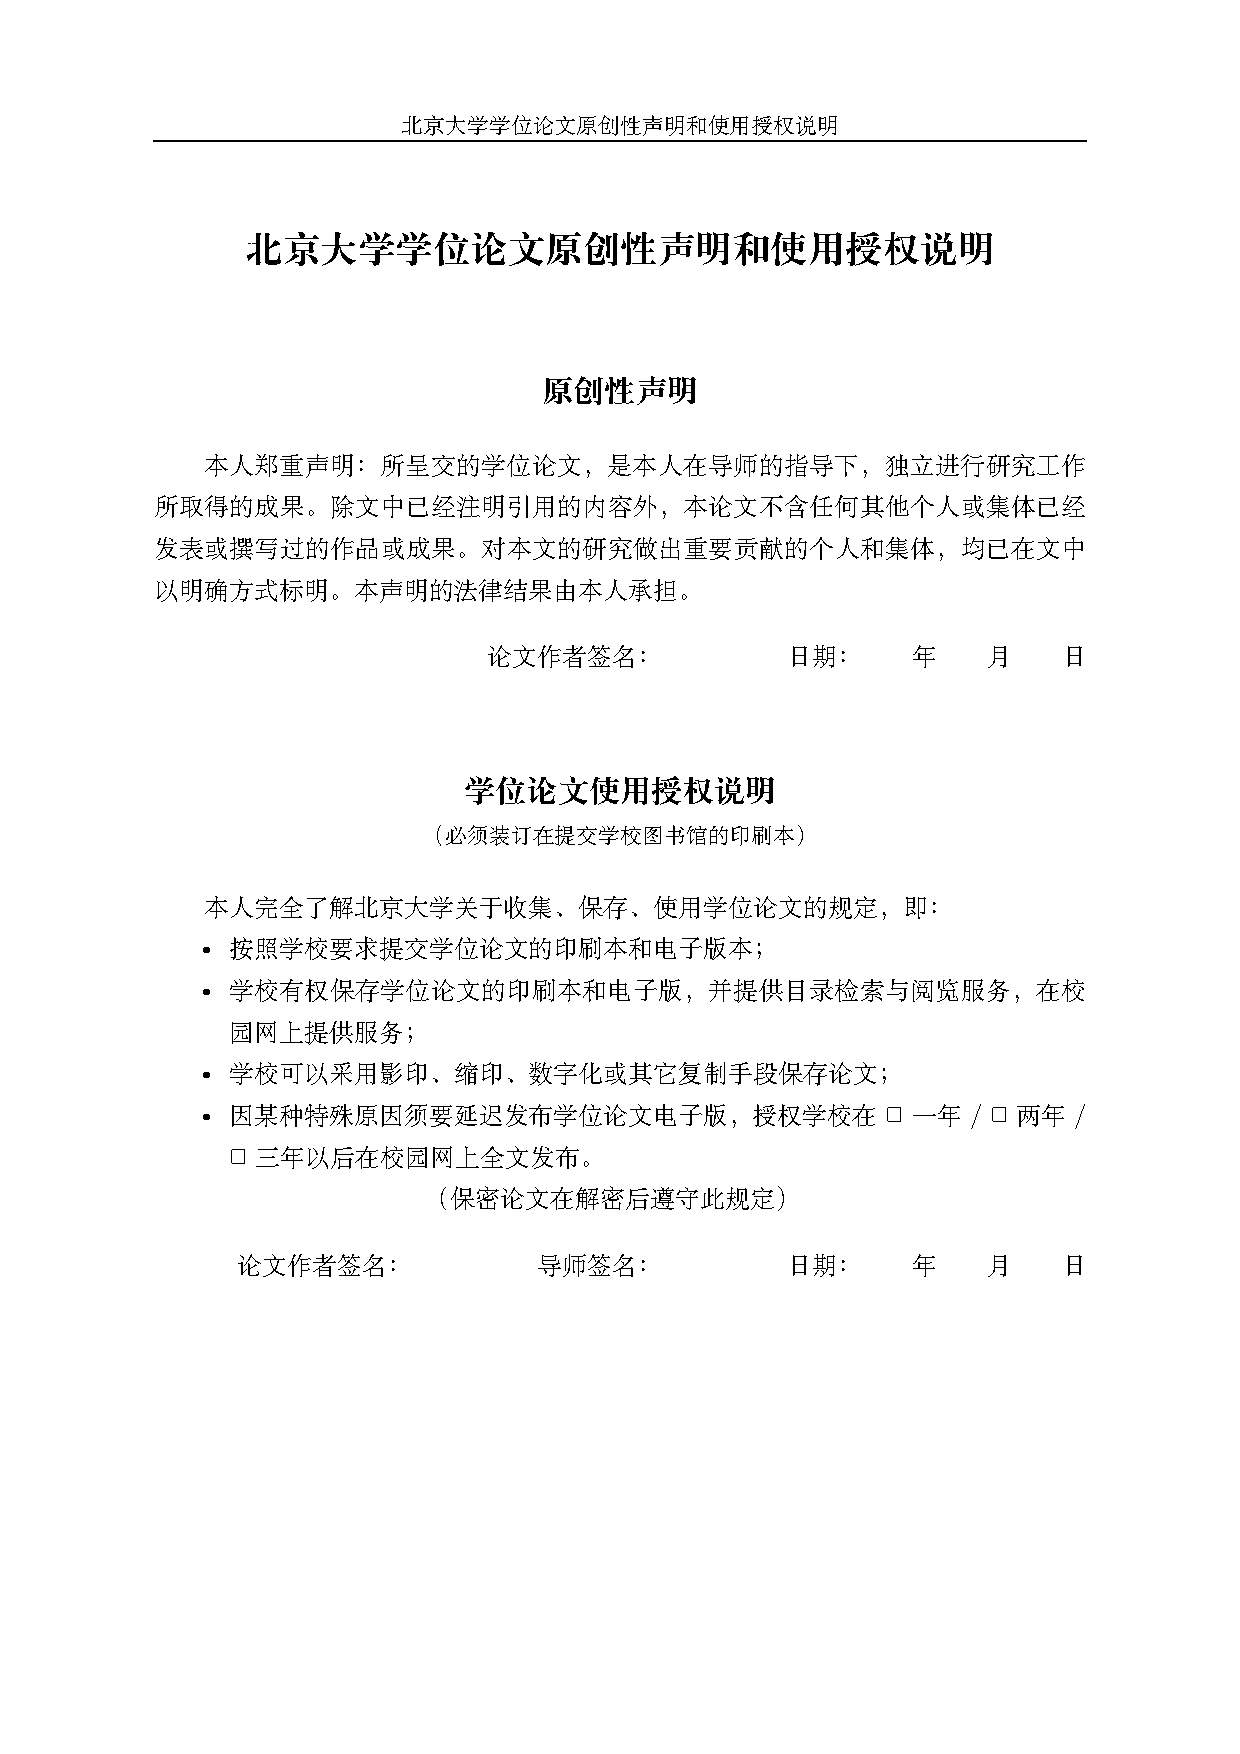
\includegraphics[height = 1.2448\textheight]{lwsm.pdf}
    }
\end{textblock}

	% 答辩后需要添加答辩委员会名单、决议书、承诺书等,在答辩前可将此行代码注释
	\ctexset{section = {
	format+ = {\centering}, beforeskip = {40bp}, afterskip = {15bp}
}}
\specialchap{学位论文答辩委员会名单}
% 替换门户下载pdf,这里用版权声明代替,你需要换成学位论文答辩委员会名单
\begin{textblock}{1}(-0.8,-0.08)
    \colorbox{white}{
        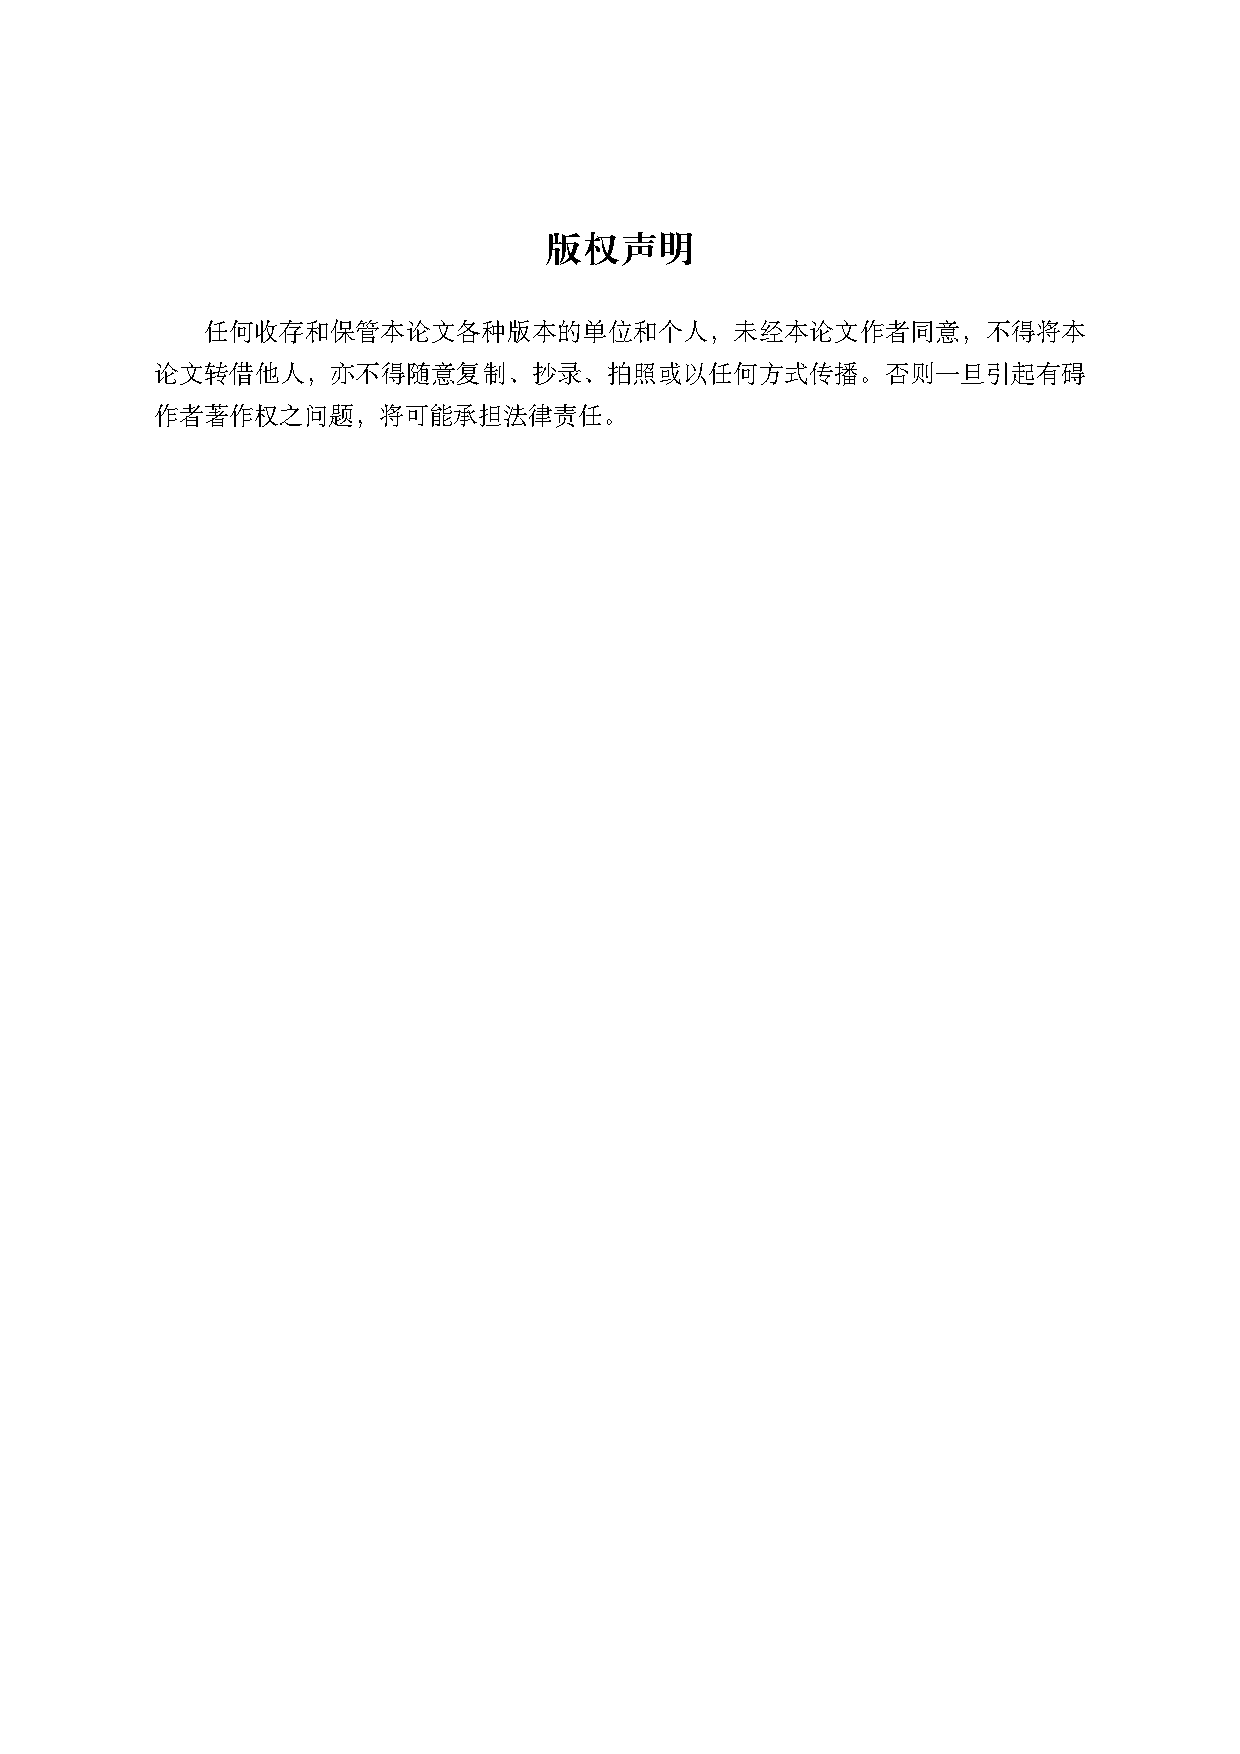
\includegraphics[height = 1.2448\textheight]{bqsm.pdf}
    }
\end{textblock}

\ctexset{section = {
	format+ = {\centering}, beforeskip = {40bp}, afterskip = {15bp}
}}
\specialchap{北京大学博士学位论文答辩委员会决议书}
% 替换门户下载pdf,这里用版权声明代替,你需要换成博士学位论文答辩委员会决议书
\begin{textblock}{1}(-0.8,-0.08)
    \colorbox{white}{
        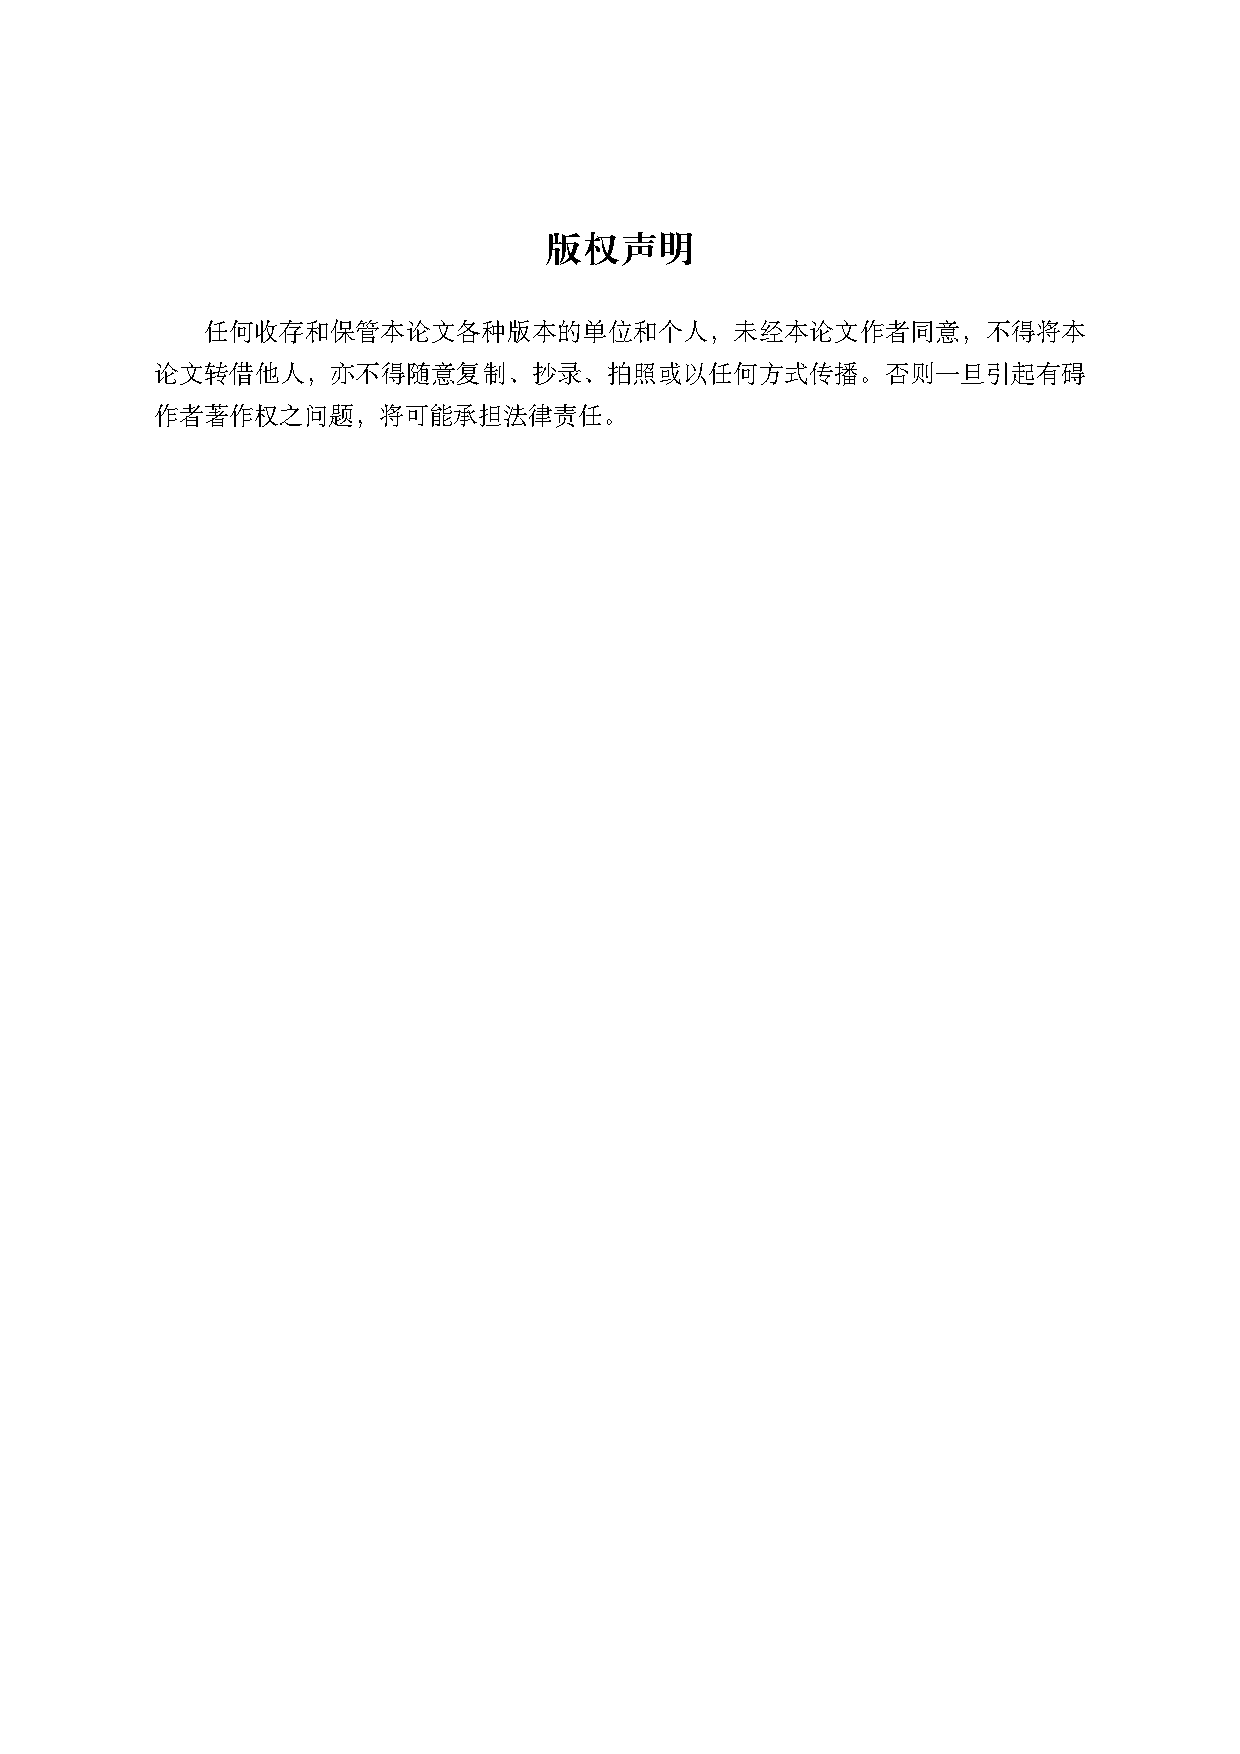
\includegraphics[height = 1.2448\textheight]{bqsm.pdf}
    }
\end{textblock}

\ctexset{section = {
	format+ = {\centering}, beforeskip = {40bp}, afterskip = {15bp}
}}
\specialchap{提交终版学位论文承诺书}
% 替换门户下载pdf,这里用版权声明代替,你需要换成提交终版学位论文承诺书
\begin{textblock}{1}(-0.8,-0.08)
    \colorbox{white}{
        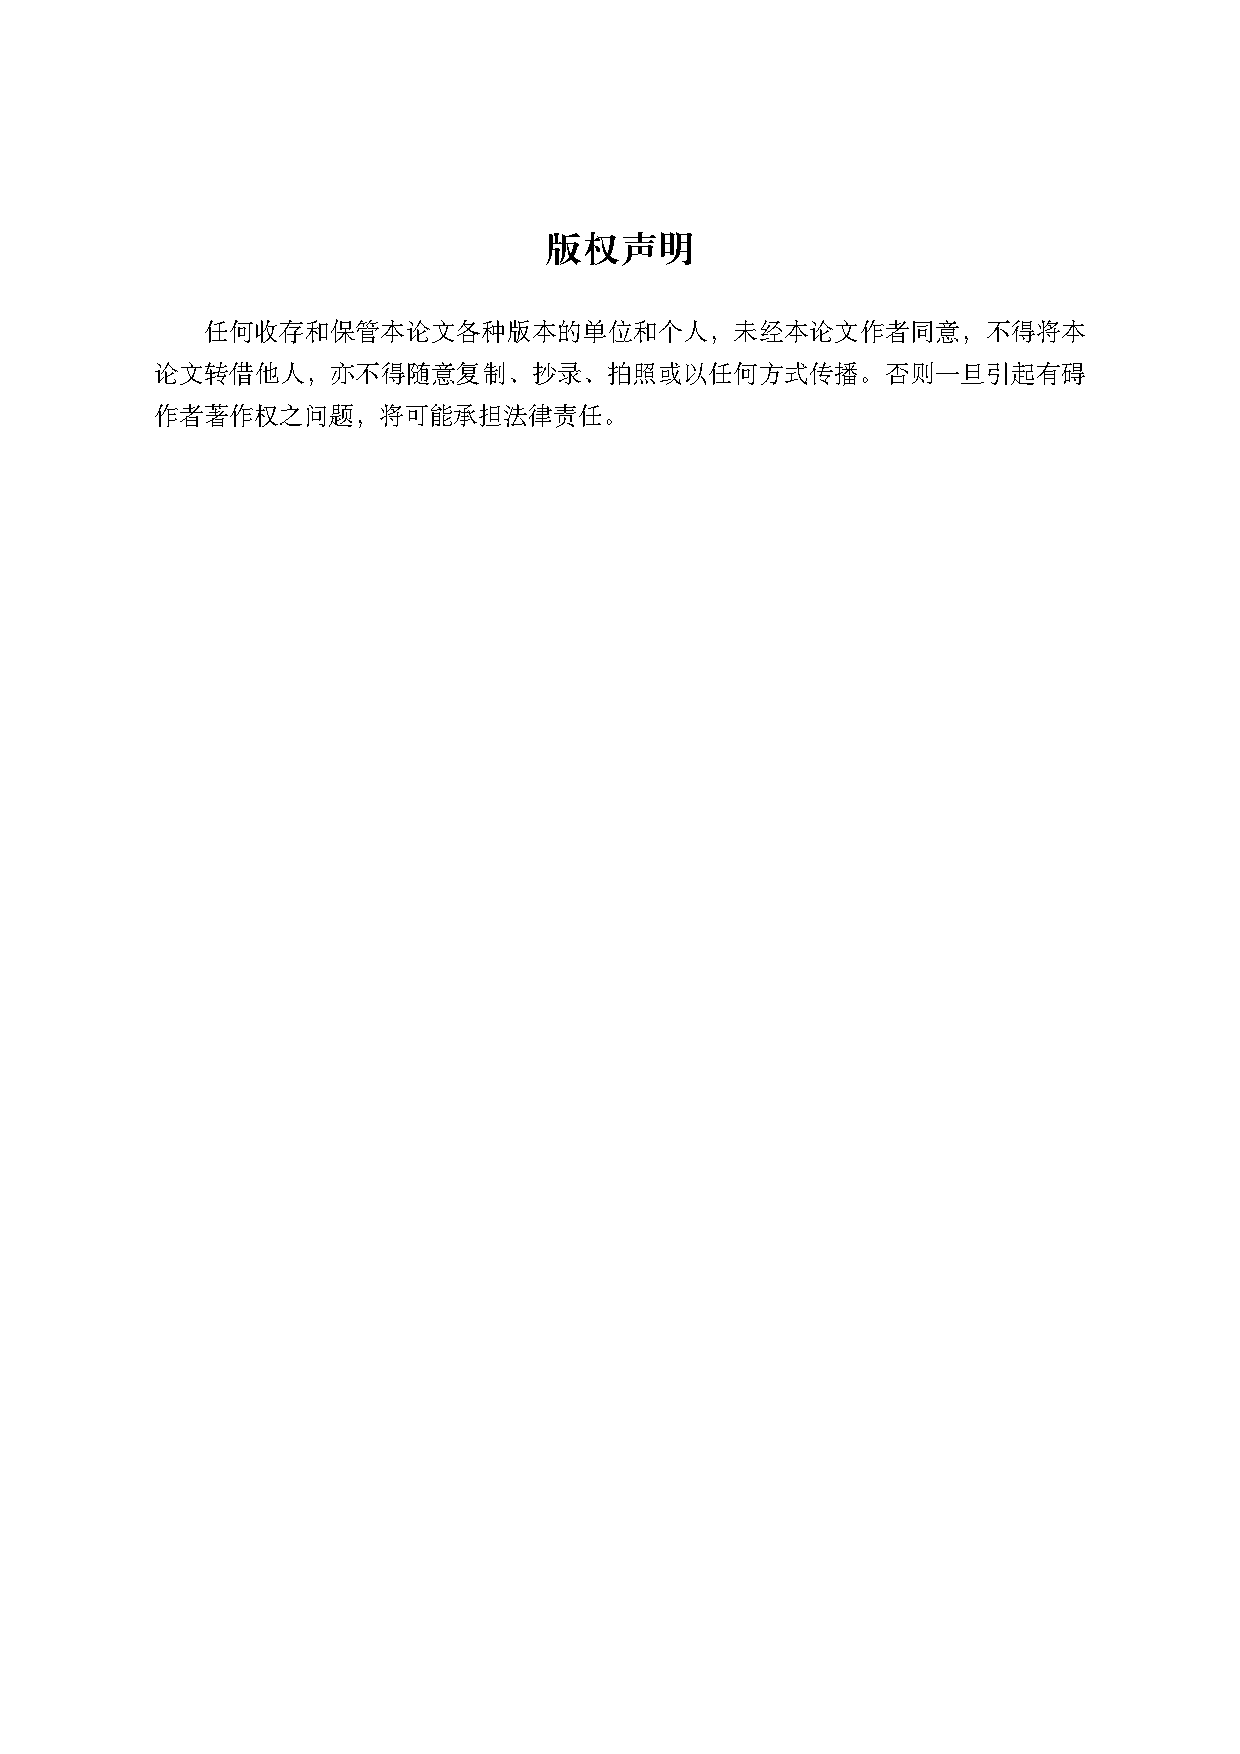
\includegraphics[height = 1.2448\textheight]{bqsm.pdf}
    }
\end{textblock}

\end{document}
